\documentclass[aspectratio=169]{beamer}
\usetheme{Madrid}
\usecolortheme{seahorse}
\usepackage{amsmath}
\usepackage{amssymb}
\usepackage{tikz}
\usepackage{algorithm}
\usepackage{algpseudocode}
\usepackage{xcolor}
\usepackage{tcolorbox}
\usepackage{pgfplots}     % This automatically loads the 'tikz' package
\pgfplotsset{compat=1.18} % Good practice for pgfplots
\usepackage{amsmath}      % For the 'align*' environment
\usetikzlibrary{shapes.geometric, arrows.meta, positioning, calc, patterns}

\pgfplotsset{compat=1.17}

% Custom colors
\definecolor{highDcolor}{RGB}{46, 134, 171}
\definecolor{lowDcolor}{RGB}{162, 59, 114}
\definecolor{gradcolor}{RGB}{255, 127, 14}

% Add these color definitions in the preamble (after line 16)
\definecolor{gray30}{gray}{0.3}
\definecolor{gray50}{gray}{0.5}
\definecolor{gray70}{gray}{0.7}

% Custom commands
\newcommand{\conceptbox}[2]{\colorbox{#1!20}{\textcolor{#1}{\textbf{#2}}}}
\newcommand{\warning}[1]{\conceptbox{red}{Warning: #1}}
\newcommand{\insight}[1]{\conceptbox{blue}{Insight: #1}}
\newcommand{\ethics}[1]{\conceptbox{purple}{Ethics: #1}}

\title{t-Stochastic Neighbor Embedding}
\subtitle{Complete 80-Slide Presentation}
\author{Prof.Asc. Endri Raco}
\institute{Polytechnic University of Tirane}
\date{October 2025}

\begin{document}

% ============================================
% SLIDES 1-10: Introduction and Fundamentals
% ============================================

% Slide 1
\begin{frame}
\titlepage
\end{frame}

\begin{frame}{What is Dimensionality Reduction?}
\begin{block}{Definition}
Transforming high-dimensional data into lower-dimensional representations while preserving meaningful structure
\end{block}

\textbf{Why We Need It:}
\begin{itemize}
\item Visualization: Human perception limited to 3D
\item Curse of dimensionality: Distance becomes meaningless in high-D
\item Computational efficiency: Reduce processing requirements
\item Feature extraction: Identify essential patterns
\end{itemize}

\textbf{The Central Challenge:}
\begin{center}
\Large How do we decide what to preserve when we must lose information?
\end{center}

\begin{columns}
\column{0.5\textwidth}
\centering
Traditional answer: \textcolor{blue}{Preserve distances}

\column{0.5\textwidth}
\centering
t-SNE answer: \textcolor{red}{Preserve neighborhoods}
\end{columns}
\end{frame}

% Slide 2
\begin{frame}{The Fundamental Challenge of Dimensionality Reduction}
\begin{columns}
\column{0.5\textwidth}
\begin{center}
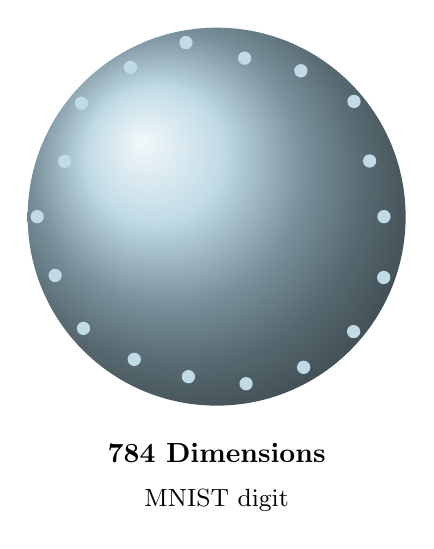
\begin{tikzpicture}[scale=1.2]
\shade[ball color=highDcolor!40] (0,0) circle (2cm);
\foreach \angle in {0,20,...,340} {
    \pgfmathsetmacro\radius{1.7+0.2*rnd}
    \fill[white!70!highDcolor] (\angle:\radius) circle (2pt);
}
\node at (0,-2.5) {\textbf{784 Dimensions}};
\node at (0,-3) {\small MNIST digit};
\end{tikzpicture}
\end{center}

\column{0.5\textwidth}
\begin{center}
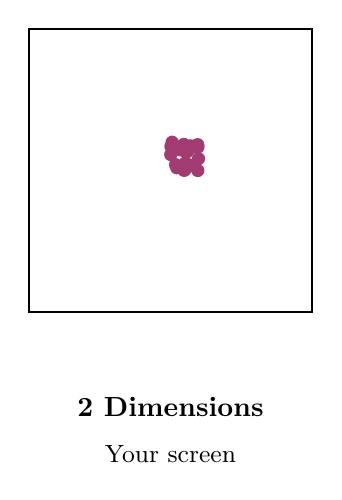
\begin{tikzpicture}[scale=1.2]
\draw[thick] (-1.5,-1.5) rectangle (1.5,1.5);
\foreach \i in {1,...,30} {
    \pgfmathsetmacro\x{0.3*rnd}
    \pgfmathsetmacro\y{0.3*rnd}
    \fill[lowDcolor] (\x,\y) circle (2pt);
}
\node at (0,-2.5) {\textbf{2 Dimensions}};
\node at (0,-3) {\small Your screen};
\end{tikzpicture}
\end{center}
\end{columns}

\vspace{0.5cm}
\begin{center}
\Large\textbf{How do we preserve neighborhood relationships \\ when destroying geometric structure?}
\end{center}
\end{frame}


% Slide 3
\begin{frame}{The Crowding Problem: Why Linear Methods Fail}
\begin{block}{Definition}
\textbf{Crowding Problem:} The geometric impossibility of preserving moderate-range distances when projecting from high to low dimensions, causing distinct distance scales to collapse.
\end{block}

\begin{columns}
\column{0.5\textwidth}
\begin{center}
\textbf{High-D Space (10D)}\\[0.2cm]
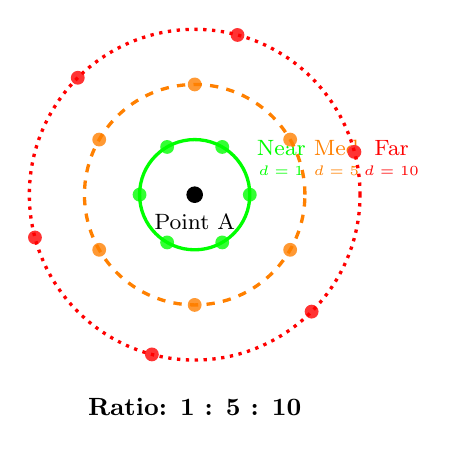
\begin{tikzpicture}[scale=1.0]
% Center point
\fill[black] (0,0) circle (3pt);
\node at (0,-0.35) {\footnotesize Point A};

% Near neighbors (distance = 1)
\foreach \angle in {0,60,120,180,240,300} {
    \fill[green!80] (\angle:0.7) circle (2.5pt);
}
\draw[green, very thick] (0,0) circle (0.7);
\node[green] at (1.1,0.6) {\footnotesize Near};
\node[green] at (1.1,0.3) {\tiny $d=1$};

% Moderate neighbors (distance = 5)
\foreach \angle in {30,90,150,210,270,330} {
    \fill[orange!80] (\angle:1.4) circle (2.5pt);
}
\draw[orange, very thick, dashed] (0,0) circle (1.4);
\node[orange] at (1.8,0.6) {\footnotesize Med};
\node[orange] at (1.8,0.3) {\tiny $d=5$};

% Far neighbors (distance = 10)
\foreach \angle in {15,75,135,195,255,315} {
    \fill[red!80] (\angle:2.1) circle (2.5pt);
}
\draw[red, very thick, dotted] (0,0) circle (2.1);
\node[red] at (2.5,0.6) {\footnotesize Far};
\node[red] at (2.5,0.3) {\tiny $d=10$};

\node at (0,-2.7) {\small\textbf{Ratio: 1 : 5 : 10}};
\end{tikzpicture}
\end{center}

\column{0.5\textwidth}
\begin{center}
\textbf{After Linear Projection to 2D}\\[0.2cm]
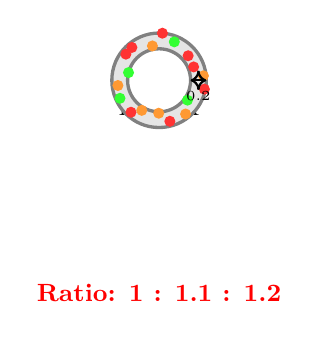
\begin{tikzpicture}[scale=1.0]
% Center point
\fill[black] (0,0) circle (3pt);
\node at (0,-0.35) {\footnotesize Point A};

% All points crushed into narrow ring
\draw[gray, very thick, fill=gray!20] (0,0) circle (0.6);
\draw[gray, very thick, fill=white] (0,0) circle (0.4);

% Mixed points in narrow annulus
\foreach \i in {1,...,18} {
    \pgfmathsetmacro\r{0.4 + 0.2*rnd}
    \pgfmathsetmacro\a{20*\i + 10*rnd}
    \pgfmathsetmacro\colorChoice{int(rnd*3)}
    \ifnum\colorChoice=0
        \fill[green!80] (\a:\r) circle (2pt);
    \fi
    \ifnum\colorChoice=1
        \fill[orange!80] (\a:\r) circle (2pt);
    \fi
    \ifnum\colorChoice=2
        \fill[red!80] (\a:\r) circle (2pt);
    \fi
}

% Show compressed distances
\draw[<->, thick] (0.4,0) -- (0.6,0);
\node at (0.5,-0.2) {\tiny 0.2};

\node at (0,-2.7) {\small\textbf{\textcolor{red}{Ratio: 1 : 1.1 : 1.2}}};
\end{tikzpicture}
\end{center}
\end{columns}

\vspace{0.15cm}
\textbf{Key Insight:} Available "area" in 2D cannot accommodate the exponentially growing "volume" of moderate distances from high-D space.
\end{frame}

% Slide 4
\begin{frame}{The Paradigm Shift: From Geometry to Information}
\begin{center}
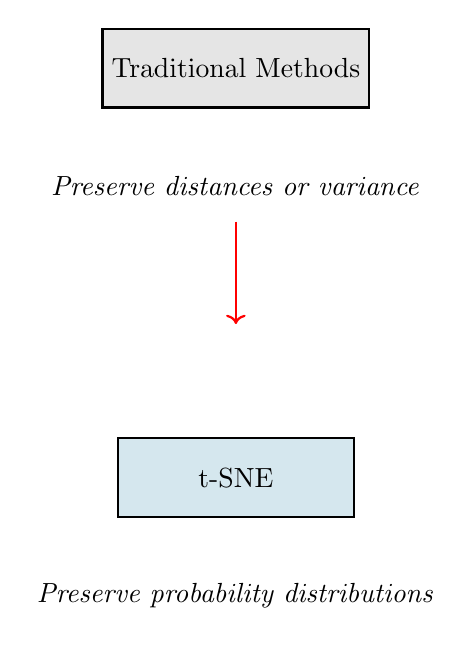
\begin{tikzpicture}[scale=1.3]
\node[draw, thick, fill=gray!20, minimum width=3cm, minimum height=1cm] (trad) at (0,3) {Traditional Methods};
\node[below of=trad, yshift=-0.5cm] {\textit{Preserve distances or variance}};
\draw[thick, red, ->] (0,1.5) -- (0,0.5);

\node[draw, thick, fill=highDcolor!20, minimum width=3cm, minimum height=1cm] (tsne) at (0,-1) {t-SNE};
\node[below of=tsne, yshift=-0.5cm] {\textit{Preserve probability distributions}};
\end{tikzpicture}
\end{center}

\vspace{0.3cm}
\begin{block}{Key Insight}
Instead of asking "How close are points?" we ask "How likely are they neighbors?"
\end{block}
\end{frame}


% Slide 5b - IMPROVED AESTHETIC VERSION
\begin{frame}{The Paradigm Shift: Concrete Example}
\begin{columns}
\column{0.5\textwidth}
\begin{tcolorbox}[colback=blue!5, colframe=blue!40, title={\textbf{Traditional: Preserve Distances}}]
\begin{center}
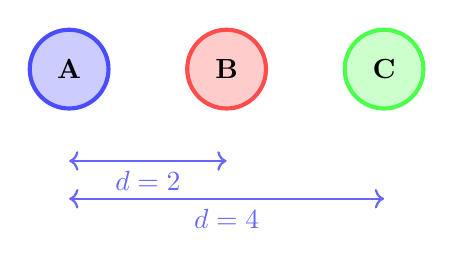
\begin{tikzpicture}[scale=0.8]
% Three points with better styling
\node[circle, draw=blue!70, fill=blue!20, line width=1.5pt, minimum size=10mm] (A) at (0,0) {\textbf{A}};
\node[circle, draw=red!70, fill=red!20, line width=1.5pt, minimum size=10mm] (B) at (2.5,0) {\textbf{B}};
\node[circle, draw=green!70, fill=green!20, line width=1.5pt, minimum size=10mm] (C) at (5,0) {\textbf{C}};

% Distance arcs
\draw[<->, thick, blue!60] ([yshift=-8mm]A.south) -- ([yshift=-8mm]B.south) node[midway, below] {$d=2$};
\draw[<->, thick, blue!60] ([yshift=-14mm]A.south) -- ([yshift=-14mm]C.south) node[midway, below] {$d=4$};
\end{tikzpicture}
\end{center}
\vspace{3mm}
\textcolor{red!70}{Problem:} All distances treated equally\\
\textcolor{gray}{No context about local density}
\end{tcolorbox}

\column{0.5\textwidth}
\begin{tcolorbox}[colback=green!5, colframe=green!40, title={\textbf{t-SNE: Preserve Probabilities}}]
\begin{center}
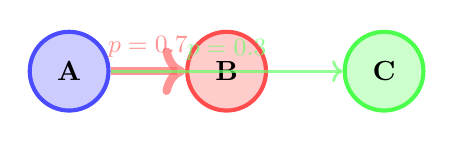
\begin{tikzpicture}[scale=0.8]
% Three points with probability visualization
\node[circle, draw=blue!70, fill=blue!20, line width=1.5pt, minimum size=10mm] (A) at (0,0) {\textbf{A}};
\node[circle, draw=red!70, fill=red!20, line width=1.5pt, minimum size=10mm] (B) at (2.5,0) {\textbf{B}};
\node[circle, draw=green!70, fill=green!20, line width=1.5pt, minimum size=10mm] (C) at (5,0) {\textbf{C}};

% Probability arrows with varying thickness
\draw[->, line width=3pt, red!60, opacity=0.7] (A) -- (B) node[midway, above] {\small $p=0.7$};
\draw[->, line width=1pt, green!60, opacity=0.7] (A) -- (C) node[midway, above] {\small $p=0.3$};
\end{tikzpicture}
\end{center}
\vspace{3mm}
\textcolor{green!70}{Solution:} Likelihood encodes context\\
\textcolor{gray}{Adapts to local density automatically}
\end{tcolorbox}
\end{columns}

\vspace{0.5cm}
\begin{tcolorbox}[colback=yellow!10, colframe=orange!60, boxrule=1pt]
\centering
\textbf{Key Insight:} Same distance $\rightarrow$ different probabilities based on neighborhood density
\end{tcolorbox}
\end{frame}


\begin{frame}{Building Intuition: From Distances to Neighborhoods}
\begin{columns}
\column{0.5\textwidth}
\textbf{The Problem with Raw Distances:}
\begin{itemize}
\item Point A: 1 unit from B, 10 units from C
\item But what if A is in dense region?
\item And C is in sparse region?
\item Raw distance loses context!
\end{itemize}

\vspace{0.3cm}
\textbf{The Solution - Relative Similarity:}
\begin{itemize}
\item Convert distances to probabilities
\item "How likely is B to be A's neighbor?"
\item Adapt to local density automatically
\item Use Gaussian decay (smooth, differentiable)
\end{itemize}

\column{0.5\textwidth}
\begin{center}
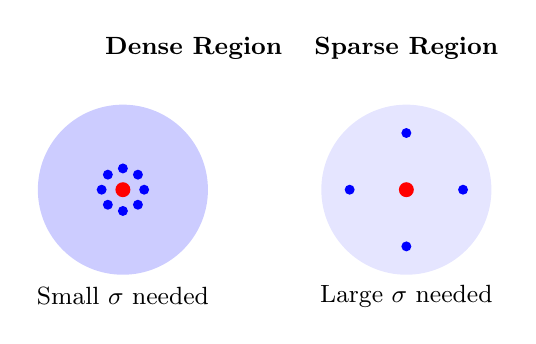
\begin{tikzpicture}[scale=0.9]
% Dense region example
\node at (0,2) {\small\textbf{Dense Region}};
\fill[blue!20] (-1,0) circle (1.2);
\fill[red] (-1,0) circle (3pt);
\foreach \angle in {0,45,...,315} {
    \fill[blue] (-1,0) ++(\angle:0.3) circle (2pt);
}
\node at (-1,-1.5) {\small Small $\sigma$ needed};

% Sparse region example  
\node at (3,2) {\small\textbf{Sparse Region}};
\fill[blue!10] (3,0) circle (1.2);
\fill[red] (3,0) circle (3pt);
\foreach \angle in {0,90,180,270} {
    \fill[blue] (3,0) ++(\angle:0.8) circle (2pt);
}
\node at (3,-1.5) {\small Large $\sigma$ needed};
\end{tikzpicture}
\end{center}

\vspace{0.2cm}
\textbf{Key Idea:} Each point gets its own "neighborhood size" ($\sigma_i$) based on local density
\end{columns}
\end{frame}

% Slide 5
\begin{frame}{From Distances to Probabilities}
\begin{columns}
\column{0.5\textwidth}
\begin{center}
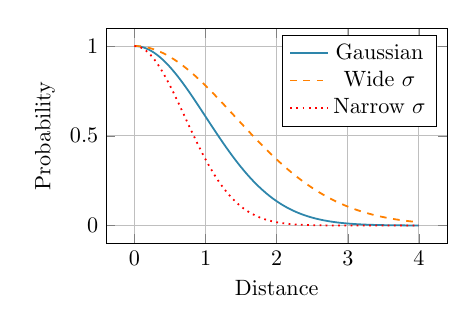
\begin{tikzpicture}[scale=0.8]
\begin{axis}[
    xlabel={Distance},
    ylabel={Probability},
    width=7cm,
    height=5cm,
    grid=major,
    legend pos=north east
]
\addplot[domain=0:4, samples=100, thick, highDcolor] {exp(-x^2/2)};
\addlegendentry{Gaussian}
\addplot[domain=0:4, samples=100, thick, orange, dashed] {exp(-x^2/4)};
\addlegendentry{Wide $\sigma$}
\addplot[domain=0:4, samples=100, thick, red, dotted] {exp(-x^2/1)};
\addlegendentry{Narrow $\sigma$}
\end{axis}
\end{tikzpicture}
\end{center}

\column{0.5\textwidth}
\textbf{Key Transformation:}
$$p_{j|i} = \frac{\exp(-\|x_i - x_j\|^2/2\sigma_i^2)}{\sum_{k \neq i} \exp(-\|x_i - x_k\|^2/2\sigma_i^2)}$$

\vspace{0.3cm}
\insight{$\sigma_i$ adapts to local density automatically}
\end{columns}
\end{frame}


% Slide 6a - INTUITIVE VERSION
\begin{frame}{Why Gaussian? The Natural Choice for Neighborhoods}
\begin{columns}
\column{0.5\textwidth}
\begin{tcolorbox}[colback=blue!5, colframe=blue!40, title={\textbf{What We're Building}}]
\textbf{Our Goal:}
\begin{itemize}
\item Convert distances to probabilities
\item "How likely is j to be i's neighbor?"
\item Must adapt to local density
\end{itemize}

\vspace{3mm}
\textbf{Three Key Requirements:}
\begin{enumerate}
\item \textcolor{blue}{Smooth decay} - no sudden cutoffs
\item \textcolor{green}{Local focus} - neighbors matter most
\item \textcolor{red}{Unbiased} - don't assume patterns
\end{enumerate}

\vspace{3mm}
\textbf{The Winner: Gaussian}
\vspace{-2mm}
$p_{j|i} \propto e^{-d_{ij}^2/2\sigma_i^2}$
\end{tcolorbox}

\column{0.5\textwidth}
\begin{center}
\textbf{Visual Comparison}\\[3mm]
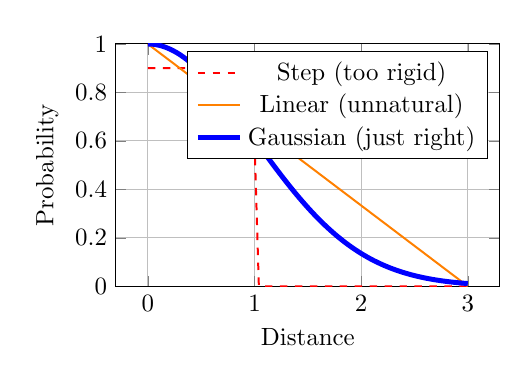
\begin{tikzpicture}[scale=0.9]
\begin{axis}[
    width=7cm,
    height=5cm,
    xlabel={Distance},
    ylabel={Probability},
    legend pos=north east,
    grid=major,
    ymin=0, ymax=1
]
% Step function - too rigid
\addplot[domain=0:3, samples=50, thick, red, dashed] {0.9*(x<1)};
\addlegendentry{Step (too rigid)}

% Linear - unnatural
\addplot[domain=0:3, samples=50, thick, orange] {max(0, 1-x/3)};
\addlegendentry{Linear (unnatural)}

% Gaussian - just right
\addplot[domain=0:3, samples=100, thick, blue, line width=2pt] {exp(-x^2/2)};
\addlegendentry{Gaussian (just right)}
\end{axis}
\end{tikzpicture}
\end{center}

\vspace{3mm}
\begin{tcolorbox}[colback=green!5, colframe=green!40, boxrule=0.5pt]
\centering\small
\textbf{Analogy:} Friendship strength\\
strongest nearby, fading smoothly
\end{tcolorbox}
\end{columns}
\end{frame}

% Slide 6b - MATHEMATICAL PRINCIPLE
\begin{frame}{The Mathematics Behind Gaussian: Maximum Entropy Principle}
\begin{columns}
\column{0.55\textwidth}
\begin{tcolorbox}[colback=yellow!5, colframe=orange!40, title={\textbf{The Core Principle}}]
\textbf{The Question:}\\
Which distribution makes the \textit{fewest assumptions} while matching our constraints?

\vspace{4mm}
\textbf{Answer: Maximum Entropy}\\
The distribution with highest uncertainty (entropy) given the constraints

\vspace{4mm}
\textbf{Why This Matters:}
\begin{itemize}
\item Most "honest" - no hidden bias
\item Adds no assumptions
\item Principled approach
\end{itemize}
\end{tcolorbox}

\column{0.45\textwidth}
\begin{center}
\textbf{Entropy Comparison}\\[3mm]
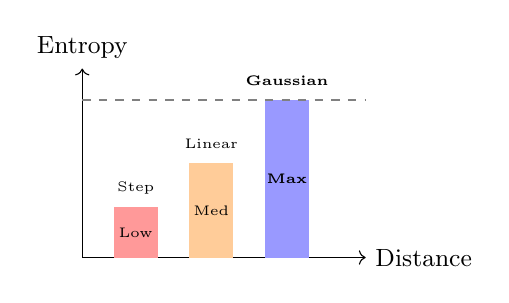
\begin{tikzpicture}[scale=0.8]
\draw[->] (0,0) -- (4.5,0) node[right] {\small Distance};
\draw[->] (0,0) -- (0,3) node[above] {\small Entropy};

% Bars showing entropy levels
\fill[red!40] (0.5,0) rectangle (1.2,0.8);
\node at (0.85,1.1) {\tiny Step};
\node at (0.85,0.4) {\tiny Low};

\fill[orange!40] (1.7,0) rectangle (2.4,1.5);
\node at (2.05,1.8) {\tiny Linear};
\node at (2.05,0.75) {\tiny Med};

\fill[blue!40] (2.9,0) rectangle (3.6,2.5);
\node at (3.25,2.8) {\tiny \textbf{Gaussian}};
\node at (3.25,1.25) {\tiny \textbf{Max}};

\draw[dashed, gray] (0,2.5) -- (4.5,2.5);
\end{tikzpicture}
\end{center}

\vspace{3mm}
\begin{tcolorbox}[colback=blue!5, colframe=blue!40]
\centering\small
\textbf{Gaussian = Maximum Entropy}\\
Most uncertain = Least biased
\end{tcolorbox}
\end{columns}
\end{frame}

% --- SLIDE 1: The Optimization Problem ---
\begin{frame}{The Mathematical Derivation: Problem Setup}
    \begin{tcolorbox}[colback=yellow!5, colframe=orange!40, title={\textbf{Optimization Problem}}]
    \textbf{Maximize Entropy:}
    \[H(P_i) = -\sum_j p_{j|i} \log p_{j|i}\]

    \textbf{Subject to Constraints:}
    \begin{enumerate}
    \item Normalization: $\sum_j p_{j|i} = 1$
    \item Fixed Variance: $\sum_j p_{j|i} d_{ij}^2 = \sigma_i^2$
    \end{enumerate}
    
    \vspace{2mm}
    \textit{The goal is to find the most unbiased probability distribution ($p_{j|i}$) that meets our constraints.}
    \end{tcolorbox}
\end{frame}


% --- SLIDE 2: The Solution ---
\begin{frame}{The Mathematical Derivation: Solution}
    \begin{tcolorbox}[colback=blue!5, colframe=blue!40, title={\textbf{Solution via Lagrange Multipliers}}]
    
    \textbf{1. The Lagrangian:}
    \begin{align*}
    \mathcal{L} = H(P_i) &+ \lambda \left(\sum p_{j|i} - 1\right) \\
                         &+ \mu \left(\sum p_{j|i}d_{ij}^2 - \sigma_i^2\right)
    \end{align*}
    
    \vspace{1mm}
    \textbf{2. Taking derivatives and solving for $\frac{\partial \mathcal{L}}{\partial p_{j|i}} = 0$ yields the result.}
    \vspace{1mm}
    
    \textbf{3. Result (The Gaussian Distribution):}
    \[
    p_{j|i} = \frac{e^{-\frac{d_{ij}^2}{2\sigma_i^2}}}{\sum_k e^{-\frac{d_{ik}^2}{2\sigma_i^2}}}
    \]
    
    \end{tcolorbox}
\end{frame}


% Slide 7 - REVISED VERSION
\begin{frame}{Perplexity: Setting the Neighborhood Size}
\begin{columns}
\column{0.5\textwidth}
\begin{tcolorbox}[colback=blue!5, colframe=blue!40, title={\textbf{The Problem We're Solving}}]
\textbf{Question:} How many neighbors should each point consider?

\vspace{3mm}
\textbf{Challenge:} Different regions have different densities!
\begin{itemize}
\item Dense areas: Small $\sigma$ needed
\item Sparse areas: Large $\sigma$ needed
\end{itemize}

\vspace{3mm}
\textbf{Solution:} Perplexity - a user parameter that sets "effective" number of neighbors
\end{tcolorbox}

\column{0.5\textwidth}
\begin{center}
\textbf{Adaptive Neighborhoods}\\[3mm]
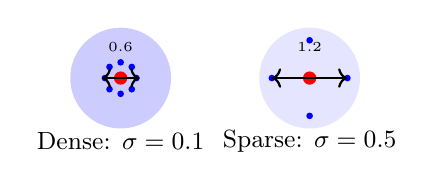
\begin{tikzpicture}[scale=0.8]
% Dense region
\fill[blue!20] (-1,1) circle (0.8);
\fill[red] (-1,1) circle (3pt);
\foreach \angle in {0,45,...,315} {
    \fill[blue] (-1,1) ++(\angle:0.25) circle (1.5pt);
}
\node at (-1,0) {\small Dense: $\sigma = 0.1$};
\draw[<->, thick] (-1.3,1) -- (-0.7,1);
\node at (-1,1.5) {\tiny 0.6};

% Sparse region  
\fill[blue!10] (2,1) circle (0.8);
\fill[red] (2,1) circle (3pt);
\foreach \angle in {0,90,180,270} {
    \fill[blue] (2,1) ++(\angle:0.6) circle (1.5pt);
}
\node at (2,0) {\small Sparse: $\sigma = 0.5$};
\draw[<->, thick] (1.4,1) -- (2.6,1);
\node at (2,1.5) {\tiny 1.2};
\end{tikzpicture}

\vspace{3mm}
\begin{tcolorbox}[colback=green!5, colframe=green!40]
\centering\small
Both have same perplexity = 5\\
Different $\sigma$ values!
\end{tcolorbox}
\end{center}
\end{columns}

\vspace{1mm}
\begin{tcolorbox}[colback=yellow!10, colframe=orange!60]
\centering
\textbf{Key Insight:} Perplexity is constant across all points, but $\sigma_i$ adapts to achieve it
\end{tcolorbox}
\end{frame}

% Slide 7b - MATHEMATICAL DEFINITION AND BINARY SEARCH
\begin{frame}{Perplexity: The Mathematics and Algorithm}
\begin{columns}
\column{0.5\textwidth}
\begin{tcolorbox}[colback=blue!5, colframe=blue!40, title={\textbf{Mathematical Definition}}]
\textbf{From Shannon Entropy:}
$$H(P_i) = -\sum_j p_{j|i} \log_2 p_{j|i}$$

\vspace{2mm}
\textbf{Perplexity:}
$$\text{Perp}(P_i) = 2^{H(P_i)}$$

\vspace{1mm}
\textbf{Interpretation:}
\begin{itemize}
\item Perp = 5 → "acts like" 5 neighbors
\item Perp = 30 → "acts like" 30 neighbors
\item Typical range: 5-50
\end{itemize}

\small\textit{Note: It's the exponential of entropy!}
\end{tcolorbox}

\column{0.5\textwidth}
\begin{tcolorbox}[colback=orange!5, colframe=orange!40, title={\textbf{Finding $\sigma_i$: Binary Search}}]
\small
\textbf{Why Binary Search?}\\
Perplexity increases with $\sigma$ monotonically

\vspace{2mm}
\begin{center}
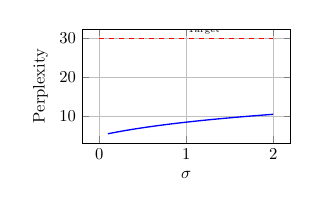
\begin{tikzpicture}[scale=0.6]
\begin{axis}[
    width=6cm,
    height=4cm,
    xlabel={$\sigma$},
    ylabel={Perplexity},
    grid=major
]
\addplot[domain=0.1:2, samples=50, thick, blue] {5*ln(x+1)+5};
\addplot[dashed, red] coordinates {(0,30) (2,30)};
\node at (axis cs:1.2,32) {\tiny Target};
\end{axis}
\end{tikzpicture}
\end{center}

\textbf{Algorithm:}
\begin{enumerate}
\item Start with $\sigma = 1$
\item Compute current perplexity
\item Too high? → Decrease $\sigma$
\item Too low? → Increase $\sigma$
\item Repeat until converged
\end{enumerate}
\normalsize
\end{tcolorbox}
\end{columns}
\end{frame}


% Slide 8 - REVISED VERSION
\begin{frame}{Measuring Information Loss: KL Divergence}
\vspace{-3mm}
\begin{columns}
\column{0.55\textwidth}
\begin{block}{What is KL Divergence?}
$$\text{KL}(P||Q) = \sum_j p_j \log\frac{p_j}{q_j}$$
\small
\textit{Extra bits needed when using $Q$ instead of true $P$}
\end{block}

\vspace{2mm}
\begin{block}{Critical Asymmetry Example}
\small
Consider point B with true probability 0.3:\\[2mm]
\textcolor{red}{\textbf{Missing a true neighbor:}}\\
True: $p = 0.3$, Embedded: $q = 0.01$\\
Penalty: $0.3 \times \log(30) \approx \textbf{1.02 bits}$\\[2mm]

\textcolor{blue}{\textbf{Creating a false neighbor:}}\\
True: $p = 0.01$, Embedded: $q = 0.3$\\
Penalty: $0.01 \times \log(0.033) \approx \textbf{-0.035 bits}$
\end{block}

\column{0.45\textwidth}
\begin{center}
\textbf{Visual Example}\\[2mm]
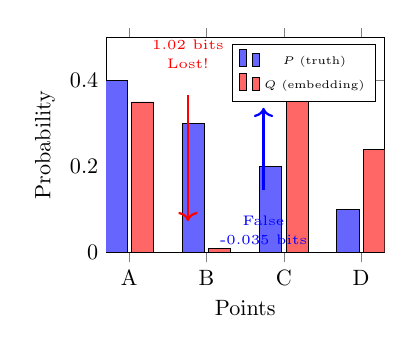
\begin{tikzpicture}[scale=0.8]
\begin{axis}[
  ybar,
  width=6cm,
  height=5cm,
  ylabel={Probability},
  xlabel={Points},
  symbolic x coords={A,B,C,D},
  xtick=data,
  ymin=0, ymax=0.5,
  legend pos=north east,
  legend style={font=\tiny}
]
\addplot[fill=blue!60] coordinates {(A,0.4) (B,0.3) (C,0.2) (D,0.1)};
\addplot[fill=red!60] coordinates {(A,0.35) (B,0.01) (C,0.4) (D,0.24)};
\legend{$P$ (truth), $Q$ (embedding)}
\end{axis}

% Annotations showing penalties
\draw[->, thick, red] (1.3, 2.5) -- (1.3, 0.5);
\node[red] at (1.3, 3) {\tiny Lost!};
\node[red] at (1.3, 3.3) {\tiny 1.02 bits};

\draw[->, thick, blue] (2.5, 1) -- (2.5, 2.3);
\node[blue] at (2.5, 0.5) {\tiny False};
\node[blue] at (2.5, 0.2) {\tiny -0.035 bits};
\end{tikzpicture}
\end{center}
\end{columns}

\vspace{2mm}
\begin{center}
\colorbox{yellow!20}{\parbox{0.9\textwidth}{\centering
\textbf{Key Insight:} t-SNE heavily penalizes separating true neighbors (30× more than false neighbors!)}}
\end{center}
\end{frame}



% Slide 9a - CONCEPTUAL INTRODUCTION
\begin{frame}{Original SNE: The Precursor to t-SNE}
\begin{center}
\textbf{A Brief History of Dimension Reduction}
\end{center}

\vspace{5mm}
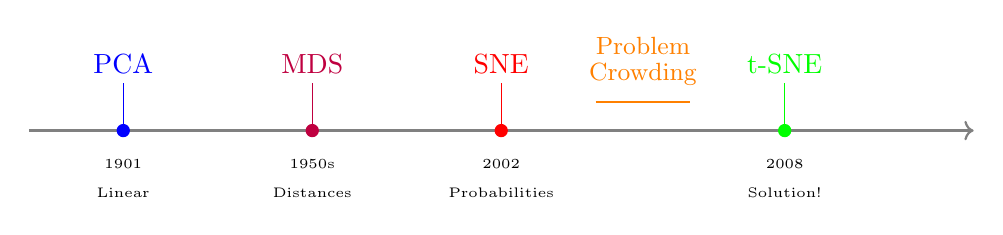
\begin{tikzpicture}[scale=1.2]
% Timeline
\draw[thick, ->, gray] (0,0) -- (10,0);

% PCA
\fill[blue] (1,0) circle (2pt);
\draw[blue] (1,0) -- (1,0.5);
\node[above, blue] at (1,0.5) {PCA};
\node[below] at (1,-0.2) {\tiny 1901};
\node[below] at (1,-0.5) {\tiny Linear};

% MDS
\fill[purple] (3,0) circle (2pt);
\draw[purple] (3,0) -- (3,0.5);
\node[above, purple] at (3,0.5) {MDS};
\node[below] at (3,-0.2) {\tiny 1950s};
\node[below] at (3,-0.5) {\tiny Distances};

% SNE
\fill[red] (5,0) circle (2pt);
\draw[red] (5,0) -- (5,0.5);
\node[above, red] at (5,0.5) {SNE};
\node[below] at (5,-0.2) {\tiny 2002};
\node[below] at (5,-0.5) {\tiny Probabilities};

% Problem
\draw[orange, thick] (6,0.3) -- (7,0.3);
\node[orange] at (6.5,0.6) {\small Crowding};
\node[orange] at (6.5,0.9) {\small Problem};

% t-SNE
\fill[green] (8,0) circle (2pt);
\draw[green] (8,0) -- (8,0.5);
\node[above, green] at (8,0.5) {t-SNE};
\node[below] at (8,-0.2) {\tiny 2008};
\node[below] at (8,-0.5) {\tiny Solution!};
\end{tikzpicture}

\vspace{8mm}
\begin{columns}
\column{0.5\textwidth}
\begin{block}{SNE's Innovation}
\begin{itemize}
\item First to use probabilities
\item Adaptive neighborhoods ($\sigma_i$)
\item Information-theoretic approach
\item KL divergence for optimization
\end{itemize}
\end{block}

\column{0.5\textwidth}
\begin{block}{SNE's Fatal Flaw}
\begin{itemize}
\item Used Gaussian in low-D space
\item Cannot represent moderate distances
\item Led to "crowding problem"
\item All points collapse together
\end{itemize}
\end{block}
\end{columns}

\vspace{1mm}
\begin{center}
\colorbox{yellow!20}{\parbox{0.9\textwidth}{\centering
\textbf{Key Lesson:} Great ideas can fail on one crucial detail}}
\end{center}
\end{frame}


\begin{frame}{SNE's Mathematics: Where It Went Wrong}
% --- 2. Use [T] to top-align the columns ---
\begin{columns}[T]

    % --- Left Column: The Formulation ---
    \column{0.5\textwidth}
\begin{block}{The Formulation}
    \begin{itemize}
        \item \textbf{High-D Similarity ($P$):} \\
              Gaussian with adaptive variance $\sigma_i$
              $$ p_{j|i} = \frac{\exp(-d_{ij}^2/2\sigma_i^2)}{\sum_k \exp(-d_{ik}^2/2\sigma_i^2)} $$

        \item \textbf{Low-D Similarity ($Q$):} \\
              \alert{Gaussian with fixed variance}
              $$ q_{j|i} = \frac{\exp(-d_{ij}^2)}{\sum_k \exp(-d_{ik}^2)} $$

        % CORRECTED LINE: The formula is now inline to save vertical space.
        \item \textbf{Cost Function:} $C = \sum_i \mathrm{KL}(P_i || Q_i)$
    \end{itemize}
\end{block}

% --- Right Column: The Problem in 2D ---
\column{0.5\textwidth}
\begin{block}{Why Gaussian Fails in 2D}
    \centering % Center the plot
    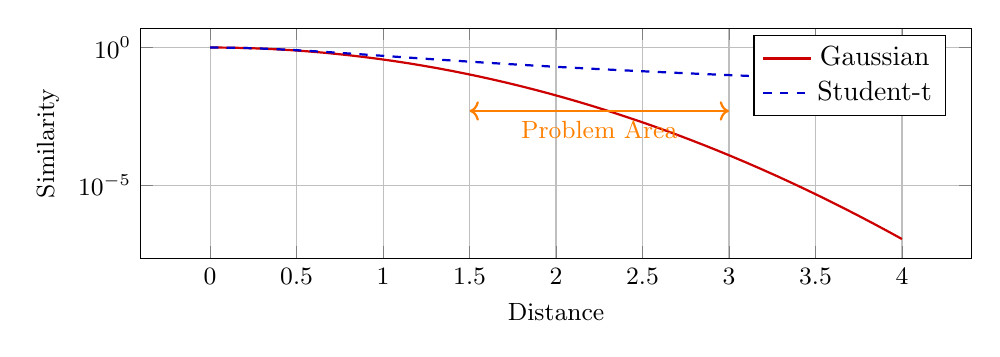
\begin{tikzpicture}
        \begin{axis}[
            width=\linewidth,
            height=4.5cm, % CORRECTED: Reduced height from 5cm
            xlabel={Distance},
            ylabel={Similarity},
            ymode=log,
            grid=major,
            legend pos=north east,
            label style={font=\small},
            tick label style={font=\small}
        ]
        \addplot[domain=0:4, samples=50, thick, red!80!black] {exp(-x^2)};
        \addlegendentry{Gaussian}
        
        \addplot[domain=0:4, samples=50, thick, blue!80!black, dashed] {1/(1+x^2)};
        \addlegendentry{Student-t}
        
        \draw[<->, orange, thick] (axis cs:1.5, 5e-3) -- (axis cs:3, 5e-3)
            node[midway, below, font=\small] {Problem Area};
        \end{axis}
    \end{tikzpicture}
    \small
    \alert{Problem:} Moderate distances in high-D get exponentially tiny similarities in low-D, causing crowding.
\end{block}

\end{columns}


\end{frame}

% Slide 10 - REVISED VERSION
\begin{frame}{The Curse: Why High-D Breaks Our Intuition}
\vspace{-3mm}
\begin{columns}
\column{0.5\textwidth}
\begin{block}{The Volume Problem}
\textbf{Question:} In a D-dimensional sphere,\\
what fraction of volume is in the outer\\
shell (radius 0.9 to 1.0)?

\vspace{3mm}
\textbf{Your intuition (2D):}
$$\frac{\pi \cdot 1^2 - \pi \cdot 0.9^2}{\pi \cdot 1^2} = 19\%$$

\textbf{Reality in high-D:}
\begin{itemize}
\item 5D: 41\%
\item 10D: 65\%
\item 50D: 99.5\%
\item \textcolor{red}{\textbf{100D: 99.997\%}}
\end{itemize}
\end{block}

\column{0.5\textwidth}
\begin{center}
\textbf{Volume Distribution by Dimension}\\[2mm]
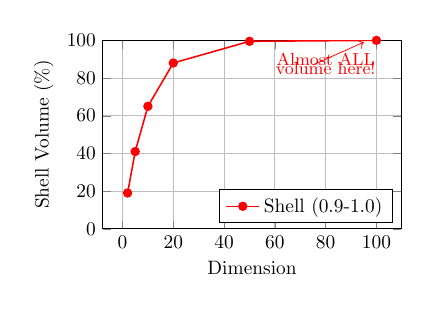
\begin{tikzpicture}[scale=0.7]
\begin{axis}[
  xlabel={Dimension},
  ylabel={Shell Volume (\%)},
  width=7cm,
  height=5cm,
  grid=major,
  ymin=0, ymax=100,
  legend pos=south east
]
\addplot[mark=*, thick, red, mark size=2pt] coordinates {
  (2,19) (5,41) (10,65) (20,88) (50,99.5) (100,99.997)
};
\addlegendentry{Shell (0.9-1.0)}

% Highlight the key point
\draw[red, very thick] (axis cs:100,99.997) circle (0.3);
\node[red] at (axis cs:80,90) {\small Almost ALL};
\node[red] at (axis cs:80,85) {\small volume here!};
\draw[red, ->] (axis cs:75,87) -- (axis cs:95,99);
\end{axis}
\end{tikzpicture}
\end{center}
\end{columns}

\vspace{3mm}
\begin{center}
\colorbox{orange!20}{\parbox{0.9\textwidth}{\centering
\textbf{Connection to SNE:} In high-D, all points are at similar distances (outer shell)\\
In 2D, we need room for varying distances that doesn't geometrically exist!}}
\end{center}
\end{frame}

\end{document}




\end{document}